\documentclass[11pt,compress,t,notes=noshow, xcolor=table]{beamer}
\usepackage[]{graphicx}\usepackage[]{color}
% maxwidth is the original width if it is less than linewidth
% otherwise use linewidth (to make sure the graphics do not exceed the margin)
\makeatletter
\def\maxwidth{ %
  \ifdim\Gin@nat@width>\linewidth
    \linewidth
  \else
    \Gin@nat@width
  \fi
}
\makeatother

\definecolor{fgcolor}{rgb}{0.345, 0.345, 0.345}
\newcommand{\hlnum}[1]{\textcolor[rgb]{0.686,0.059,0.569}{#1}}%
\newcommand{\hlstr}[1]{\textcolor[rgb]{0.192,0.494,0.8}{#1}}%
\newcommand{\hlcom}[1]{\textcolor[rgb]{0.678,0.584,0.686}{\textit{#1}}}%
\newcommand{\hlopt}[1]{\textcolor[rgb]{0,0,0}{#1}}%
\newcommand{\hlstd}[1]{\textcolor[rgb]{0.345,0.345,0.345}{#1}}%
\newcommand{\hlkwa}[1]{\textcolor[rgb]{0.161,0.373,0.58}{\textbf{#1}}}%
\newcommand{\hlkwb}[1]{\textcolor[rgb]{0.69,0.353,0.396}{#1}}%
\newcommand{\hlkwc}[1]{\textcolor[rgb]{0.333,0.667,0.333}{#1}}%
\newcommand{\hlkwd}[1]{\textcolor[rgb]{0.737,0.353,0.396}{\textbf{#1}}}%
\let\hlipl\hlkwb

\usepackage{framed}
\makeatletter
\newenvironment{kframe}{%
 \def\at@end@of@kframe{}%
 \ifinner\ifhmode%
  \def\at@end@of@kframe{\end{minipage}}%
  \begin{minipage}{\columnwidth}%
 \fi\fi%
 \def\FrameCommand##1{\hskip\@totalleftmargin \hskip-\fboxsep
 \colorbox{shadecolor}{##1}\hskip-\fboxsep
     % There is no \\@totalrightmargin, so:
     \hskip-\linewidth \hskip-\@totalleftmargin \hskip\columnwidth}%
 \MakeFramed {\advance\hsize-\width
   \@totalleftmargin\z@ \linewidth\hsize
   \@setminipage}}%
 {\par\unskip\endMakeFramed%
 \at@end@of@kframe}
\makeatother

\definecolor{shadecolor}{rgb}{.97, .97, .97}
\definecolor{messagecolor}{rgb}{0, 0, 0}
\definecolor{warningcolor}{rgb}{1, 0, 1}
\definecolor{errorcolor}{rgb}{1, 0, 0}
\newenvironment{knitrout}{}{} % an empty environment to be redefined in TeX

\usepackage{alltt}
\newcommand{\SweaveOpts}[1]{}  % do not interfere with LaTeX
\newcommand{\SweaveInput}[1]{} % because they are not real TeX commands
\newcommand{\Sexpr}[1]{}       % will only be parsed by R
\newcommand{\xmark}{\ding{55}}%


\usepackage[english]{babel}
\usepackage[utf8]{inputenc}

\usepackage{dsfont}
\usepackage{verbatim}
\usepackage{amsmath}
\usepackage{amsfonts}
\usepackage{amssymb}
\usepackage{bm}
\usepackage{csquotes}
\usepackage{multirow}
\usepackage{longtable}
\usepackage{booktabs}
\usepackage{enumerate}
\usepackage[absolute,overlay]{textpos}
\usepackage{psfrag}
\usepackage{algorithm}
\usepackage{algpseudocode}
\usepackage{eqnarray}
\usepackage{arydshln}
\usepackage{tabularx}
\usepackage{placeins}
\usepackage{tikz}
\usepackage{setspace}
\usepackage{colortbl}
\usepackage{mathtools}
\usepackage{wrapfig}
\usepackage{bm}
\usepackage{amsmath}
\usepackage{pifont}
\usepackage[round]{natbib}
\usepackage{hyperref}

\usetikzlibrary{shapes,arrows,automata,positioning,calc,chains,trees, shadows}
\tikzset{
  %Define standard arrow tip
  >=stealth',
  %Define style for boxes
  punkt/.style={
    rectangle,
    rounded corners,
    draw=black, very thick,
    text width=6.5em,
    minimum height=2em,
    text centered},
  % Define arrow style
  pil/.style={
    ->,
    thick,
    shorten <=2pt,
    shorten >=2pt,}
}

\usepackage{subfig}

% Defines macros and environments
\usepackage{../../style/lmu-lecture}


\let\code=\texttt
\let\proglang=\textsf

\setkeys{Gin}{width=0.9\textwidth}

\setbeamertemplate{frametitle}{\expandafter\uppercase\expandafter\insertframetitle}

% basic latex stuff
\newcommand{\pkg}[1]{{\fontseries{b}\selectfont #1}} % fontstyle for R packages

% Often used in exercise Rnw files, still relevant?
\newcommand{\lz}{\vspace{0.5cm}} % vertical space
\newcommand{\dlz}{\vspace{1cm}}  % double vertical space

% Unused and about to be deleted
\newcommand{\oneliner}[1] % Oneliner for important statements
{\begin{block}{}\begin{center}\begin{Large}#1\end{Large}\end{center}\end{block}}


%--------------------%
%  New environments  %
%--------------------%

 % Frame with breaks and verbatim // this is used very often
\newenvironment{vbframe}
{
\begin{frame}[containsverbatim,allowframebreaks]
}
{
\end{frame}
}

% Frame with verbatim without breaks (to avoid numbering one slided frames)
% This is not used anywhere but I can see it being useful
\newenvironment{vframe}
{
\begin{frame}[containsverbatim]
}
{
\end{frame}
}

% Itemize block
\newenvironment{blocki}[1]
{
\begin{block}{#1}\begin{itemize}
}
{
\end{itemize}\end{block}
}

%--------------%
%  Citebutton  %
%--------------%
% Example usage (from slides-cart-discussion.tex)
% \citebutton{Breiman, 1984}{https://www.taylorfrancis.com/books/mono/10.1201/9781315139470/classification-regression-trees-leo-breiman}
\newcommand{\citebutton}[2]{%
\NoCaseChange{\resizebox{!}{9pt}{\protect\beamergotobutton{\href{#2}{#1}}}}%
}

% textcolor that works in mathmode
% https://tex.stackexchange.com/a/261480
% Used e.g. in forests/slides-forests-bagging.tex
% [...] \textcolor{blue}{\tfrac{1}{M}\sum^M_{m} [...]
\makeatletter
\renewcommand*{\@textcolor}[3]{%
  \protect\leavevmode
  \begingroup
    \color#1{#2}#3%
  \endgroup
}
\makeatother





% dependencies: amsmath, amssymb, dsfont
% math spaces
\ifdefined\N
\renewcommand{\N}{\mathds{N}} % N, naturals
\else \newcommand{\N}{\mathds{N}} \fi
\newcommand{\Z}{\mathds{Z}} % Z, integers
\newcommand{\Q}{\mathds{Q}} % Q, rationals
\newcommand{\R}{\mathds{R}} % R, reals
\ifdefined\C
\renewcommand{\C}{\mathds{C}} % C, complex
\else \newcommand{\C}{\mathds{C}} \fi
\newcommand{\continuous}{\mathcal{C}} % C, space of continuous functions
\newcommand{\M}{\mathcal{M}} % machine numbers
\newcommand{\epsm}{\epsilon_m} % maximum error

% counting / finite sets
\newcommand{\setzo}{\{0, 1\}} % set 0, 1
\newcommand{\setmp}{\{-1, +1\}} % set -1, 1
\newcommand{\unitint}{[0, 1]} % unit interval

% basic math stuff
\newcommand{\xt}{\tilde x} % x tilde
\DeclareMathOperator*{\argmax}{arg\,max} % argmax
\DeclareMathOperator*{\argmin}{arg\,min} % argmin
\newcommand{\argminlim}{\mathop{\mathrm{arg\,min}}\limits} % argmax with limits
\newcommand{\argmaxlim}{\mathop{\mathrm{arg\,max}}\limits} % argmin with limits
\newcommand{\sign}{\operatorname{sign}} % sign, signum
\newcommand{\I}{\mathbb{I}} % I, indicator
\newcommand{\order}{\mathcal{O}} % O, order
\newcommand{\bigO}{\mathcal{O}} % Big-O Landau
\newcommand{\littleo}{{o}} % Little-o Landau
\newcommand{\pd}[2]{\frac{\partial{#1}}{\partial #2}} % partial derivative
\newcommand{\floorlr}[1]{\left\lfloor #1 \right\rfloor} % floor
\newcommand{\ceillr}[1]{\left\lceil #1 \right\rceil} % ceiling
\newcommand{\indep}{\perp \!\!\! \perp} % independence symbol

% sums and products
\newcommand{\sumin}{\sum\limits_{i=1}^n} % summation from i=1 to n
\newcommand{\sumim}{\sum\limits_{i=1}^m} % summation from i=1 to m
\newcommand{\sumjn}{\sum\limits_{j=1}^n} % summation from j=1 to p
\newcommand{\sumjp}{\sum\limits_{j=1}^p} % summation from j=1 to p
\newcommand{\sumik}{\sum\limits_{i=1}^k} % summation from i=1 to k
\newcommand{\sumkg}{\sum\limits_{k=1}^g} % summation from k=1 to g
\newcommand{\sumjg}{\sum\limits_{j=1}^g} % summation from j=1 to g
\newcommand{\meanin}{\frac{1}{n} \sum\limits_{i=1}^n} % mean from i=1 to n
\newcommand{\meanim}{\frac{1}{m} \sum\limits_{i=1}^m} % mean from i=1 to n
\newcommand{\meankg}{\frac{1}{g} \sum\limits_{k=1}^g} % mean from k=1 to g
\newcommand{\prodin}{\prod\limits_{i=1}^n} % product from i=1 to n
\newcommand{\prodkg}{\prod\limits_{k=1}^g} % product from k=1 to g
\newcommand{\prodjp}{\prod\limits_{j=1}^p} % product from j=1 to p

% linear algebra
\newcommand{\one}{\bm{1}} % 1, unitvector
\newcommand{\zero}{\mathbf{0}} % 0-vector
\newcommand{\id}{\bm{I}} % I, identity
\newcommand{\diag}{\operatorname{diag}} % diag, diagonal
\newcommand{\trace}{\operatorname{tr}} % tr, trace
\newcommand{\spn}{\operatorname{span}} % span
\newcommand{\scp}[2]{\left\langle #1, #2 \right\rangle} % <.,.>, scalarproduct
\newcommand{\mat}[1]{\begin{pmatrix} #1 \end{pmatrix}} % short pmatrix command
\newcommand{\Amat}{\mathbf{A}} % matrix A
\newcommand{\Deltab}{\mathbf{\Delta}} % error term for vectors

% basic probability + stats
\renewcommand{\P}{\mathds{P}} % P, probability
\newcommand{\E}{\mathds{E}} % E, expectation
\newcommand{\var}{\mathsf{Var}} % Var, variance
\newcommand{\cov}{\mathsf{Cov}} % Cov, covariance
\newcommand{\corr}{\mathsf{Corr}} % Corr, correlation
\newcommand{\normal}{\mathcal{N}} % N of the normal distribution
\newcommand{\iid}{\overset{i.i.d}{\sim}} % dist with i.i.d superscript
\newcommand{\distas}[1]{\overset{#1}{\sim}} % ... is distributed as ...

% machine learning
\newcommand{\Xspace}{\mathcal{X}} % X, input space
\newcommand{\Yspace}{\mathcal{Y}} % Y, output space
\newcommand{\Zspace}{\mathcal{Z}} % Z, space of sampled datapoints
\newcommand{\nset}{\{1, \ldots, n\}} % set from 1 to n
\newcommand{\pset}{\{1, \ldots, p\}} % set from 1 to p
\newcommand{\gset}{\{1, \ldots, g\}} % set from 1 to g
\newcommand{\Pxy}{\mathbb{P}_{xy}} % P_xy
\newcommand{\Exy}{\mathbb{E}_{xy}} % E_xy: Expectation over random variables xy
\newcommand{\xv}{\mathbf{x}} % vector x (bold)
\newcommand{\xtil}{\tilde{\mathbf{x}}} % vector x-tilde (bold)
\newcommand{\yv}{\mathbf{y}} % vector y (bold)
\newcommand{\xy}{(\xv, y)} % observation (x, y)
\newcommand{\xvec}{\left(x_1, \ldots, x_p\right)^\top} % (x1, ..., xp)
\newcommand{\Xmat}{\mathbf{X}} % Design matrix
\newcommand{\allDatasets}{\mathds{D}} % The set of all datasets
\newcommand{\allDatasetsn}{\mathds{D}_n}  % The set of all datasets of size n
\newcommand{\D}{\mathcal{D}} % D, data
\newcommand{\Dn}{\D_n} % D_n, data of size n
\newcommand{\Dtrain}{\mathcal{D}_{\text{train}}} % D_train, training set
\newcommand{\Dtest}{\mathcal{D}_{\text{test}}} % D_test, test set
\newcommand{\xyi}[1][i]{\left(\xv^{(#1)}, y^{(#1)}\right)} % (x^i, y^i), i-th observation
\newcommand{\Dset}{\left( \xyi[1], \ldots, \xyi[n]\right)} % {(x1,y1)), ..., (xn,yn)}, data
\newcommand{\defAllDatasetsn}{(\Xspace \times \Yspace)^n} % Def. of the set of all datasets of size n
\newcommand{\defAllDatasets}{\bigcup_{n \in \N}(\Xspace \times \Yspace)^n} % Def. of the set of all datasets
\newcommand{\xdat}{\left\{ \xv^{(1)}, \ldots, \xv^{(n)}\right\}} % {x1, ..., xn}, input data
\newcommand{\ydat}{\left\{ \yv^{(1)}, \ldots, \yv^{(n)}\right\}} % {y1, ..., yn}, input data
\newcommand{\yvec}{\left(y^{(1)}, \hdots, y^{(n)}\right)^\top} % (y1, ..., yn), vector of outcomes
\newcommand{\greekxi}{\xi} % Greek letter xi
\renewcommand{\xi}[1][i]{\xv^{(#1)}} % x^i, i-th observed value of x
\newcommand{\yi}[1][i]{y^{(#1)}} % y^i, i-th observed value of y
\newcommand{\xivec}{\left(x^{(i)}_1, \ldots, x^{(i)}_p\right)^\top} % (x1^i, ..., xp^i), i-th observation vector
\newcommand{\xj}{\xv_j} % x_j, j-th feature
\newcommand{\xjvec}{\left(x^{(1)}_j, \ldots, x^{(n)}_j\right)^\top} % (x^1_j, ..., x^n_j), j-th feature vector
\newcommand{\phiv}{\mathbf{\phi}} % Basis transformation function phi
\newcommand{\phixi}{\mathbf{\phi}^{(i)}} % Basis transformation of xi: phi^i := phi(xi)

%%%%%% ml - models general
\newcommand{\lamv}{\bm{\lambda}} % lambda vector, hyperconfiguration vector
\newcommand{\Lam}{\bm{\Lambda}}	 % Lambda, space of all hpos
% Inducer / Inducing algorithm
\newcommand{\preimageInducer}{\left(\defAllDatasets\right)\times\Lam} % Set of all datasets times the hyperparameter space
\newcommand{\preimageInducerShort}{\allDatasets\times\Lam} % Set of all datasets times the hyperparameter space
% Inducer / Inducing algorithm
\newcommand{\ind}{\mathcal{I}} % Inducer, inducing algorithm, learning algorithm

% continuous prediction function f
\newcommand{\ftrue}{f_{\text{true}}}  % True underlying function (if a statistical model is assumed)
\newcommand{\ftruex}{\ftrue(\xv)} % True underlying function (if a statistical model is assumed)
\newcommand{\fx}{f(\xv)} % f(x), continuous prediction function
\newcommand{\fdomains}{f: \Xspace \rightarrow \R^g} % f with domain and co-domain
\newcommand{\Hspace}{\mathcal{H}} % hypothesis space where f is from
\newcommand{\fbayes}{f^{\ast}} % Bayes-optimal model
\newcommand{\fxbayes}{f^{\ast}(\xv)} % Bayes-optimal model
\newcommand{\fkx}[1][k]{f_{#1}(\xv)} % f_j(x), discriminant component function
\newcommand{\fh}{\hat{f}} % f hat, estimated prediction function
\newcommand{\fxh}{\fh(\xv)} % fhat(x)
\newcommand{\fxt}{f(\xv ~|~ \thetav)} % f(x | theta)
\newcommand{\fxi}{f\left(\xv^{(i)}\right)} % f(x^(i))
\newcommand{\fxih}{\hat{f}\left(\xv^{(i)}\right)} % f(x^(i))
\newcommand{\fxit}{f\left(\xv^{(i)} ~|~ \thetav\right)} % f(x^(i) | theta)
\newcommand{\fhD}{\fh_{\D}} % fhat_D, estimate of f based on D
\newcommand{\fhDtrain}{\fh_{\Dtrain}} % fhat_Dtrain, estimate of f based on D
\newcommand{\fhDnlam}{\fh_{\Dn, \lamv}} %model learned on Dn with hp lambda
\newcommand{\fhDlam}{\fh_{\D, \lamv}} %model learned on D with hp lambda
\newcommand{\fhDnlams}{\fh_{\Dn, \lamv^\ast}} %model learned on Dn with optimal hp lambda
\newcommand{\fhDlams}{\fh_{\D, \lamv^\ast}} %model learned on D with optimal hp lambda

% discrete prediction function h
\newcommand{\hx}{h(\xv)} % h(x), discrete prediction function
\newcommand{\hh}{\hat{h}} % h hat
\newcommand{\hxh}{\hat{h}(\xv)} % hhat(x)
\newcommand{\hxt}{h(\xv | \thetav)} % h(x | theta)
\newcommand{\hxi}{h\left(\xi\right)} % h(x^(i))
\newcommand{\hxit}{h\left(\xi ~|~ \thetav\right)} % h(x^(i) | theta)
\newcommand{\hbayes}{h^{\ast}} % Bayes-optimal classification model
\newcommand{\hxbayes}{h^{\ast}(\xv)} % Bayes-optimal classification model

% yhat
\newcommand{\yh}{\hat{y}} % yhat for prediction of target
\newcommand{\yih}{\hat{y}^{(i)}} % yhat^(i) for prediction of ith targiet
\newcommand{\resi}{\yi- \yih}

% theta
\newcommand{\thetah}{\hat{\theta}} % theta hat
\newcommand{\thetav}{\bm{\theta}} % theta vector
\newcommand{\thetavh}{\bm{\hat\theta}} % theta vector hat
\newcommand{\thetat}[1][t]{\thetav^{[#1]}} % theta^[t] in optimization
\newcommand{\thetatn}[1][t]{\thetav^{[#1 +1]}} % theta^[t+1] in optimization
\newcommand{\thetahDnlam}{\thetavh_{\Dn, \lamv}} %theta learned on Dn with hp lambda
\newcommand{\thetahDlam}{\thetavh_{\D, \lamv}} %theta learned on D with hp lambda
\newcommand{\mint}{\min_{\thetav \in \Theta}} % min problem theta
\newcommand{\argmint}{\argmin_{\thetav \in \Theta}} % argmin theta

% densities + probabilities
% pdf of x
\newcommand{\pdf}{p} % p
\newcommand{\pdfx}{p(\xv)} % p(x)
\newcommand{\pixt}{\pi(\xv~|~ \thetav)} % pi(x|theta), pdf of x given theta
\newcommand{\pixit}[1][i]{\pi\left(\xi[#1] ~|~ \thetav\right)} % pi(x^i|theta), pdf of x given theta
\newcommand{\pixii}[1][i]{\pi\left(\xi[#1]\right)} % pi(x^i), pdf of i-th x

% pdf of (x, y)
\newcommand{\pdfxy}{p(\xv,y)} % p(x, y)
\newcommand{\pdfxyt}{p(\xv, y ~|~ \thetav)} % p(x, y | theta)
\newcommand{\pdfxyit}{p\left(\xi, \yi ~|~ \thetav\right)} % p(x^(i), y^(i) | theta)

% pdf of x given y
\newcommand{\pdfxyk}[1][k]{p(\xv | y= #1)} % p(x | y = k)
\newcommand{\lpdfxyk}[1][k]{\log p(\xv | y= #1)} % log p(x | y = k)
\newcommand{\pdfxiyk}[1][k]{p\left(\xi | y= #1 \right)} % p(x^i | y = k)

% prior probabilities
\newcommand{\pik}[1][k]{\pi_{#1}} % pi_k, prior
\newcommand{\lpik}[1][k]{\log \pi_{#1}} % log pi_k, log of the prior
\newcommand{\pit}{\pi(\thetav)} % Prior probability of parameter theta

% posterior probabilities
\newcommand{\post}{\P(y = 1 ~|~ \xv)} % P(y = 1 | x), post. prob for y=1
\newcommand{\postk}[1][k]{\P(y = #1 ~|~ \xv)} % P(y = k | y), post. prob for y=k
\newcommand{\pidomains}{\pi: \Xspace \rightarrow \unitint} % pi with domain and co-domain
\newcommand{\pibayes}{\pi^{\ast}} % Bayes-optimal classification model
\newcommand{\pixbayes}{\pi^{\ast}(\xv)} % Bayes-optimal classification model
\newcommand{\pix}{\pi(\xv)} % pi(x), P(y = 1 | x)
\newcommand{\piv}{\bm{\pi}} % pi, bold, as vector
\newcommand{\pikx}[1][k]{\pi_{#1}(\xv)} % pi_k(x), P(y = k | x)
\newcommand{\pikxt}[1][k]{\pi_{#1}(\xv ~|~ \thetav)} % pi_k(x | theta), P(y = k | x, theta)
\newcommand{\pixh}{\hat \pi(\xv)} % pi(x) hat, P(y = 1 | x) hat
\newcommand{\pikxh}[1][k]{\hat \pi_{#1}(\xv)} % pi_k(x) hat, P(y = k | x) hat
\newcommand{\pixih}{\hat \pi(\xi)} % pi(x^(i)) with hat
\newcommand{\pikxih}[1][k]{\hat \pi_{#1}(\xi)} % pi_k(x^(i)) with hat
\newcommand{\pdfygxt}{p(y ~|~\xv, \thetav)} % p(y | x, theta)
\newcommand{\pdfyigxit}{p\left(\yi ~|~\xi, \thetav\right)} % p(y^i |x^i, theta)
\newcommand{\lpdfygxt}{\log \pdfygxt } % log p(y | x, theta)
\newcommand{\lpdfyigxit}{\log \pdfyigxit} % log p(y^i |x^i, theta)

% probababilistic
\newcommand{\bayesrulek}[1][k]{\frac{\P(\xv | y= #1) \P(y= #1)}{\P(\xv)}} % Bayes rule
\newcommand{\muk}{\bm{\mu_k}} % mean vector of class-k Gaussian (discr analysis)

% residual and margin
\newcommand{\eps}{\epsilon} % residual, stochastic
\newcommand{\epsv}{\bm{\epsilon}} % residual, stochastic, as vector
\newcommand{\epsi}{\epsilon^{(i)}} % epsilon^i, residual, stochastic
\newcommand{\epsh}{\hat{\epsilon}} % residual, estimated
\newcommand{\epsvh}{\hat{\epsv}} % residual, estimated, vector
\newcommand{\yf}{y \fx} % y f(x), margin
\newcommand{\yfi}{\yi \fxi} % y^i f(x^i), margin
\newcommand{\Sigmah}{\hat \Sigma} % estimated covariance matrix
\newcommand{\Sigmahj}{\hat \Sigma_j} % estimated covariance matrix for the j-th class

% ml - loss, risk, likelihood
\newcommand{\Lyf}{L\left(y, f\right)} % L(y, f), loss function
\newcommand{\Lypi}{L\left(y, \pi\right)} % L(y, pi), loss function
\newcommand{\Lxy}{L\left(y, \fx\right)} % L(y, f(x)), loss function
\newcommand{\Lxyi}{L\left(\yi, \fxi\right)} % loss of observation
\newcommand{\Lxyt}{L\left(y, \fxt\right)} % loss with f parameterized
\newcommand{\Lxyit}{L\left(\yi, \fxit\right)} % loss of observation with f parameterized
\newcommand{\Lxym}{L\left(\yi, f\left(\bm{\tilde{x}}^{(i)} ~|~ \thetav\right)\right)} % loss of observation with f parameterized
\newcommand{\Lpixy}{L\left(y, \pix\right)} % loss in classification
\newcommand{\Lpiv}{L\left(y, \piv\right)} % loss in classification
\newcommand{\Lpixyi}{L\left(\yi, \pixii\right)} % loss of observation in classification
\newcommand{\Lpixyt}{L\left(y, \pixt\right)} % loss with pi parameterized
\newcommand{\Lpixyit}{L\left(\yi, \pixit\right)} % loss of observation with pi parameterized
\newcommand{\Lhxy}{L\left(y, \hx\right)} % L(y, h(x)), loss function on discrete classes
\newcommand{\Lr}{L\left(r\right)} % L(r), loss defined on residual (reg) / margin (classif)
\newcommand{\lone}{|y - \fx|} % L1 loss
\newcommand{\ltwo}{\left(y - \fx\right)^2} % L2 loss
\newcommand{\lbernoullimp}{\ln(1 + \exp(-y \cdot \fx))} % Bernoulli loss for -1, +1 encoding
\newcommand{\lbernoullizo}{- y \cdot \fx + \log(1 + \exp(\fx))} % Bernoulli loss for 0, 1 encoding
\newcommand{\lcrossent}{- y \log \left(\pix\right) - (1 - y) \log \left(1 - \pix\right)} % cross-entropy loss
\newcommand{\lbrier}{\left(\pix - y \right)^2} % Brier score
\newcommand{\risk}{\mathcal{R}} % R, risk
\newcommand{\riskbayes}{\mathcal{R}^\ast}
\newcommand{\riskf}{\risk(f)} % R(f), risk
\newcommand{\riskdef}{\E_{y|\xv}\left(\Lxy \right)} % risk def (expected loss)
\newcommand{\riskt}{\mathcal{R}(\thetav)} % R(theta), risk
\newcommand{\riske}{\mathcal{R}_{\text{emp}}} % R_emp, empirical risk w/o factor 1 / n
\newcommand{\riskeb}{\bar{\mathcal{R}}_{\text{emp}}} % R_emp, empirical risk w/ factor 1 / n
\newcommand{\riskef}{\riske(f)} % R_emp(f)
\newcommand{\risket}{\mathcal{R}_{\text{emp}}(\thetav)} % R_emp(theta)
\newcommand{\riskr}{\mathcal{R}_{\text{reg}}} % R_reg, regularized risk
\newcommand{\riskrt}{\mathcal{R}_{\text{reg}}(\thetav)} % R_reg(theta)
\newcommand{\riskrf}{\riskr(f)} % R_reg(f)
\newcommand{\riskrth}{\hat{\mathcal{R}}_{\text{reg}}(\thetav)} % hat R_reg(theta)
\newcommand{\risketh}{\hat{\mathcal{R}}_{\text{emp}}(\thetav)} % hat R_emp(theta)
\newcommand{\LL}{\mathcal{L}} % L, likelihood
\newcommand{\LLt}{\mathcal{L}(\thetav)} % L(theta), likelihood
\newcommand{\LLtx}{\mathcal{L}(\thetav | \xv)} % L(theta|x), likelihood
\newcommand{\logl}{\ell} % l, log-likelihood
\newcommand{\loglt}{\logl(\thetav)} % l(theta), log-likelihood
\newcommand{\logltx}{\logl(\thetav | \xv)} % l(theta|x), log-likelihood
\newcommand{\errtrain}{\text{err}_{\text{train}}} % training error
\newcommand{\errtest}{\text{err}_{\text{test}}} % test error
\newcommand{\errexp}{\overline{\text{err}_{\text{test}}}} % avg training error

% lm
\newcommand{\thx}{\thetav^\top \xv} % linear model
\newcommand{\olsest}{(\Xmat^\top \Xmat)^{-1} \Xmat^\top \yv} % OLS estimator in LM

% ml - Gaussian Process

\newcommand{\fvec}{\left[f\left(\xi[1]\right), \dots, f\left(\xi[n]\right) \right]} % function vector
\newcommand{\fv}{\mathbf{f}} % function vector
\newcommand{\kv}{\mathbf{k}} % cov matrix partition
\newcommand{\kxxp}{k\left(\xv, \xv^{\prime} \right)} % cov of x, x'
\newcommand{\kxij}[2]{k\left(\xi, \xi[j] \right)} % cov of x_i, x_j
\newcommand{\mv}{\mathbf{m}} % GP mean vector
\newcommand{\Kmat}{\mathbf{K}} % GP cov matrix
\newcommand{\gaussmk}{\normal(\mv, \Kmat)} % Gaussian w/ mean vec, cov mat
\newcommand{\gp}{\mathcal{GP}\left(m(\xv), \kxxp \right)} % Gaussian Process Definition
\newcommand{\ls}{\ell} % length-scale
\newcommand{\sqexpkernel}{\exp \left(- \frac{\| \xv - \xv^{\prime} \|^2}{2 \ls^2} \right)} % squared exponential kernel

% GP prediction
\newcommand{\fstarvec}{\left[f\left(\xi[1]_{\ast}\right), \dots, f\left(\xi[m]_{\ast}\right) \right]} % pred function vector
\newcommand{\kstar}{\kv_{\ast}} % cov of new obs with x
\newcommand{\kstarstar}{\kv_{\ast \ast}} % cov of new obs
\newcommand{\Kstar}{\Kmat_{\ast}} % cov mat of new obs with x
\newcommand{\Kstarstar}{\Kmat_{\ast \ast}} % cov mat of new obs
\newcommand{\preddistsingle}{f_{\ast} ~|~ \xv_{\ast}, \Xmat, \fv} % predictive distribution for single pred
\newcommand{\preddistdefsingle}{\normal(\kstar^\top\Kmat^{-1}\fv, \kstarstar - \kstar^\top \Kmat ^{-1}\kstar)} % Gaussian distribution for single pred
\newcommand{\preddist}{f_{\ast} ~|~ \Xmat_{\ast}, \Xmat, \fv} % predictive distribution
\newcommand{\preddistdef}{\normal(\Kstar^\top\Kmat^{-1}\fv, \Kstarstar - \Kstar^\top \Kmat ^{-1}\Kstar)} % Gaussian predictive distribution


\newcommand{\titlefigure}{figure_man/post-variance.png}
\newcommand{\learninggoals}{
  \item Know how to derive the posterior process
  \item GPs are interpolating and spatial models
  \item Model noise via a nugget term
}

\title{Introduction to Machine Learning}
\date{}

\begin{document}

\lecturechapter{Gaussian Process Prediction}
\lecture{Introduction to Machine Learning}

\begin{vbframe}{Gaussian Posterior Process And Prediction}

\vspace*{1cm}

\begin{itemize}
  \item So far, we have learned how to \textbf{sample} from a GP prior.
\item However, most of the time, we are not interested in drawing random functions from the prior. Instead, we usually like to use the knowledge provided by the training data to predict values of $f$ at a new test point $\xv_*$. 
\item In what follows, we will investigate how to update the Gaussian process prior ($\to$ posterior process) and how to make predictions.
\end{itemize}

\end{vbframe}

\section{Gaussian Posterior Process and Prediction}


\begin{vbframe}{Posterior process}

% \textbf{Noise-free Case:}
% 
% In the noise-free case, $y^{(i)} = f(\xi)$ ($\epsi \equiv 0$, no additive noise). The targets correspond to the true function values $\yv = \bm{f}$ (training observations) and $\yv^* = \bm{f}^*$ (test observations).
% 
% \lz 

\begin{itemize}
  \item Let us now distinguish between observed training inputs, also denote by a design matrix $\Xmat$, and the corresponding observed values
  $$
    \bm{f} = \left[f\left(\xi[1]\right), ..., f\left(\xi[n]\right)\right]
  $$ 

and one single \textbf{unobserved test point} $\xv_*$ with $f_* = f\left(\xv_*\right).$

\item We now want to infer the distribution of $f_* | \xv_*, \bm{X}, \bm{f}$.
  $$
    f_* = f\left(\xv_*\right)
  $$  
  \item Assuming a zero-mean GP prior $\mathcal{GP}\left(\bm{0}, k(\xv, \xv^\prime)\right)$ we know

$$
\begin{bmatrix}
\bm{f} \\
f_*
\end{bmatrix} \sim  
\mathcal{N}\biggl(\bm{0}, \begin{bmatrix} \Kmat & \bm{k}_* \\ \bm{k}_*^T & \bm{k}_{**}\end{bmatrix}\biggr).
$$

Here, $\Kmat = \left(k\left(\xi, \xv^{(j)}\right)\right)_{i,j}$, $\bm{k}_* = \left[k\left(\xv_*, \xi[1]\right), ..., k\left(\xv_*, \xi[n]\right)\right]$ and $ \bm{k}_{**}\ = k(\xv_*, \xv_*)$. 

\framebreak 

\item Given that $\bm{f}$ is observed, we can apply the general rule for condition $^{(*)}$ of Gaussian random variables and obtain the following formula: 

\begin{eqnarray*}
f_* ~|~ \xv_*, \Xmat, \bm{f} \sim \mathcal{N}(\bm{k}_{*}^{T}\Kmat^{-1}\bm{f}, \bm{k}_{**} - \bm{k}_*^T \Kmat ^{-1}\bm{k}_*).
\end{eqnarray*}

% \begin{eqnarray*}
% \bm{f}_* | \Xmat_*, \Xmat, \bm{f} \sim \mathcal{N}(\Kmat_{*}^{T}\Kmat^{-1}\bm{f}, \Kmat_{**} - \Kmat_*^T \Kmat ^{-1}\Kmat_*).
% \end{eqnarray*}
\item As the posterior is a Gaussian, the maximum a-posteriori estimate, i.e. the mode of the posterior distribution, is $\bm{k}_{*}^{T}\Kmat^{-1}\bm{f}. $
\end{itemize}

\framebreak 

$^{(*)}$ General rule for condition of Gaussian random variables: 

\lz 

  If the $m$-dimensional Gaussian vector $\bm{z} \sim \mathcal{N}(\mu, \Sigma)$ can be partitioned with $\bm{z} = \left(\bm{z}_1, \bm{z}_2\right)$ where $\bm{z}_1$ is $m_1$-dimensional and $\bm{z}_2$ is $m_2$-dimensional, and:
$$\left(\mu_1, \mu_2\right), \quad \Sigma = \begin{pmatrix} \Sigma_{11} & \Sigma_{12} \\ \Sigma_{21} & \Sigma_{22} \end{pmatrix},$$

then the conditioned distribution of $\bm{z}_2 ~|~ \bm{z}_1 = \bm{a}$ is a multivariate normal  

$$
  \mathcal{N}\left(\mu_2 + \Sigma_{21} \Sigma_{11}^{-1}\left(\bm{a} - \mu_1\right), \Sigma_{22} - \Sigma_{21}\Sigma_{11}^{-1}\Sigma_{12} \right)
$$

\end{vbframe} 

\begin{frame}{GP prediction: Two points}

Let us visualize this by a simple example: 
\begin{itemize}
  \item Assume we observed a single training point $\xv = - 0.5$, and want to make a prediction at a test point $\xv_* = 0.5$. 
  \item Under a zero-mean GP with $k(\xv, \xv^\prime) = \exp(-\frac{1}{2}\|\xv - \xv^\prime\|^2)$, we compute the cov-matrix:
  $$
    \begin{bmatrix} f \\ f_* \end{bmatrix} \sim \mathcal{N}\biggl(\bm{0}, \begin{bmatrix} 1 & 0.61 \\ 0.61 & 1\end{bmatrix}\biggr). 
  $$ 
  \item Assume that we observe the point $\fx = 1$. 
  \item We compute the posterior distribution: 
  \begin{eqnarray*}
    f_* ~|~ \xv_*, \xv, f &\sim& \mathcal{N}(\bm{k}_{*}^{T}\Kmat^{-1}f, k_{**} - \bm{k}_*^T \Kmat^{-1}\bm{k}_*) \\
    &\sim& \mathcal{N}(0.61 \cdot 1 \cdot 1, 1 - 0.61 \cdot 1 \cdot 0.61) \\
    &\sim& \mathcal{N}\left(0.61, 0.6279\right) 
  \end{eqnarray*}
  \item The MAP-estimate for $\xv_*$ is $f(\xv_*) = 0.61$, and the uncertainty estimate is $0.6279$. 
  % what can we say about the function value at a new point $\xv_* = -0.5$? 
  % \item<+-> We compute the covariance function and have

  % \item<+-> After observing $\fx = 1$ we want to predict a value for $f(\xv_*)$. 
  % \item<+-> We compute the posterior distribution conditioned on $\fx = 1$
  % \begin{eqnarray*}

  % \end{eqnarray*}
\end{itemize}

\end{frame} 


\begin{vbframe}{GP prediction: Two points}

\begin{footnotesize}
  Shown is the bivariate normal density, and the respective marginals. 
\end{footnotesize}\vspace*{0.2cm}

\begin{figure}
  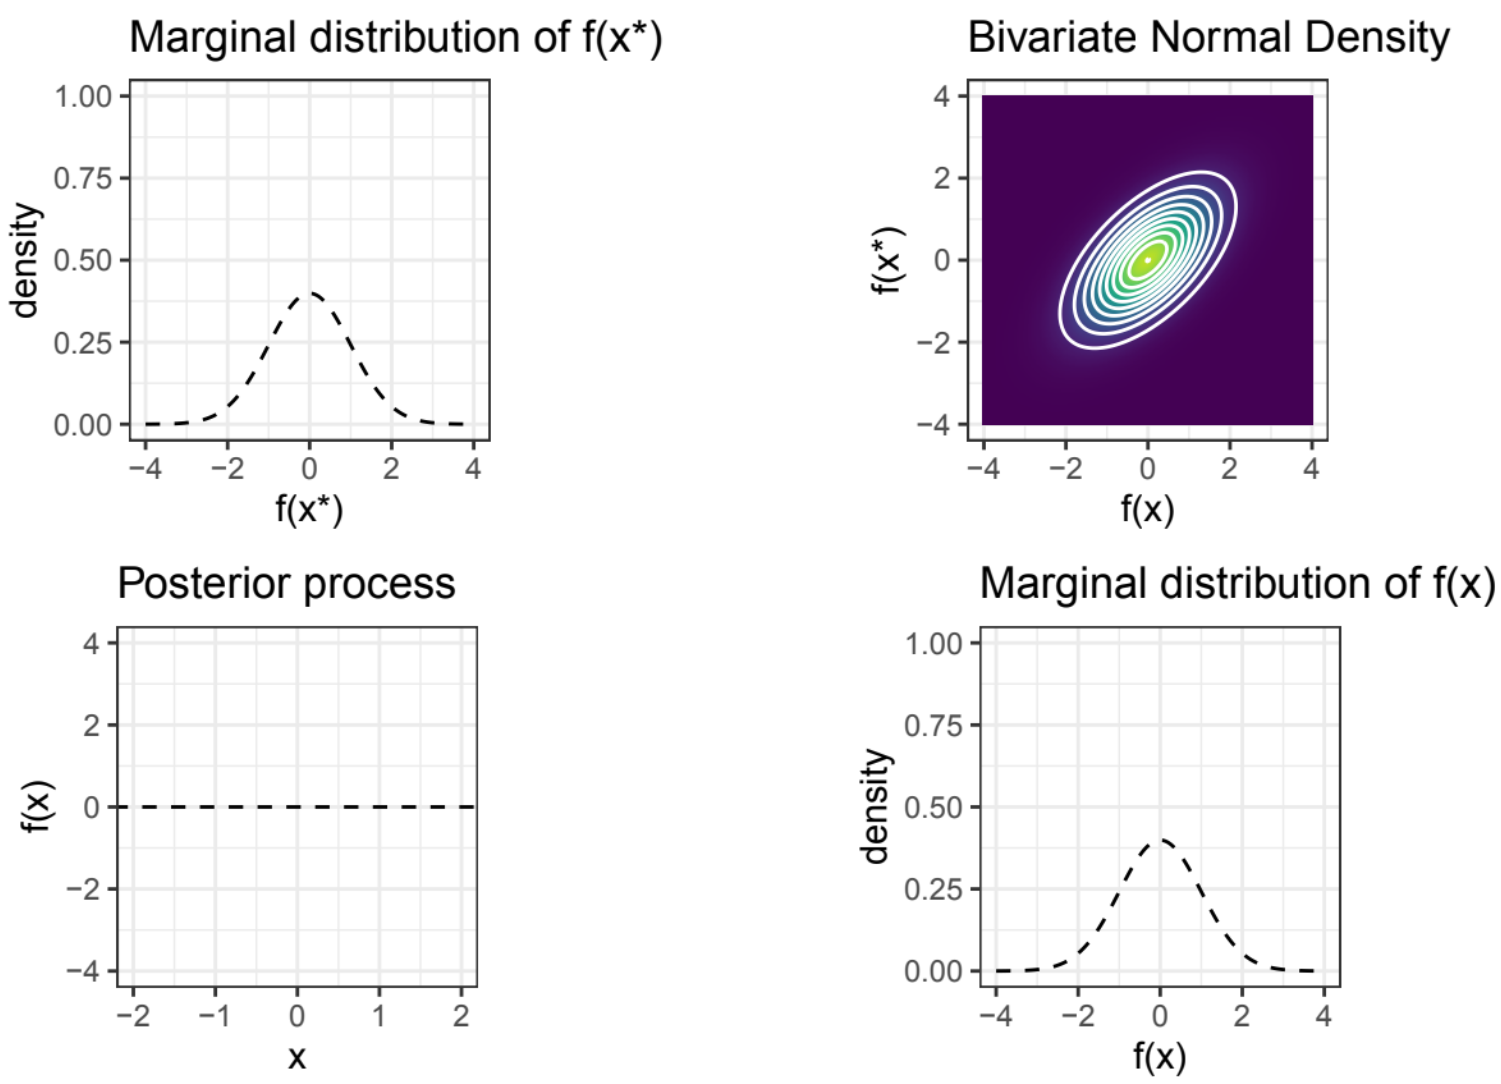
\includegraphics[width=0.8\textwidth]{figure_man/GP01.png}
\end{figure}


\end{vbframe}

\begin{frame}{GP prediction: Two points}

\begin{footnotesize}
  Assume we observed $\fx = 1$ for the training point $\xv = -0.5$.  
\end{footnotesize}\vspace*{0.2cm}

\begin{figure}
  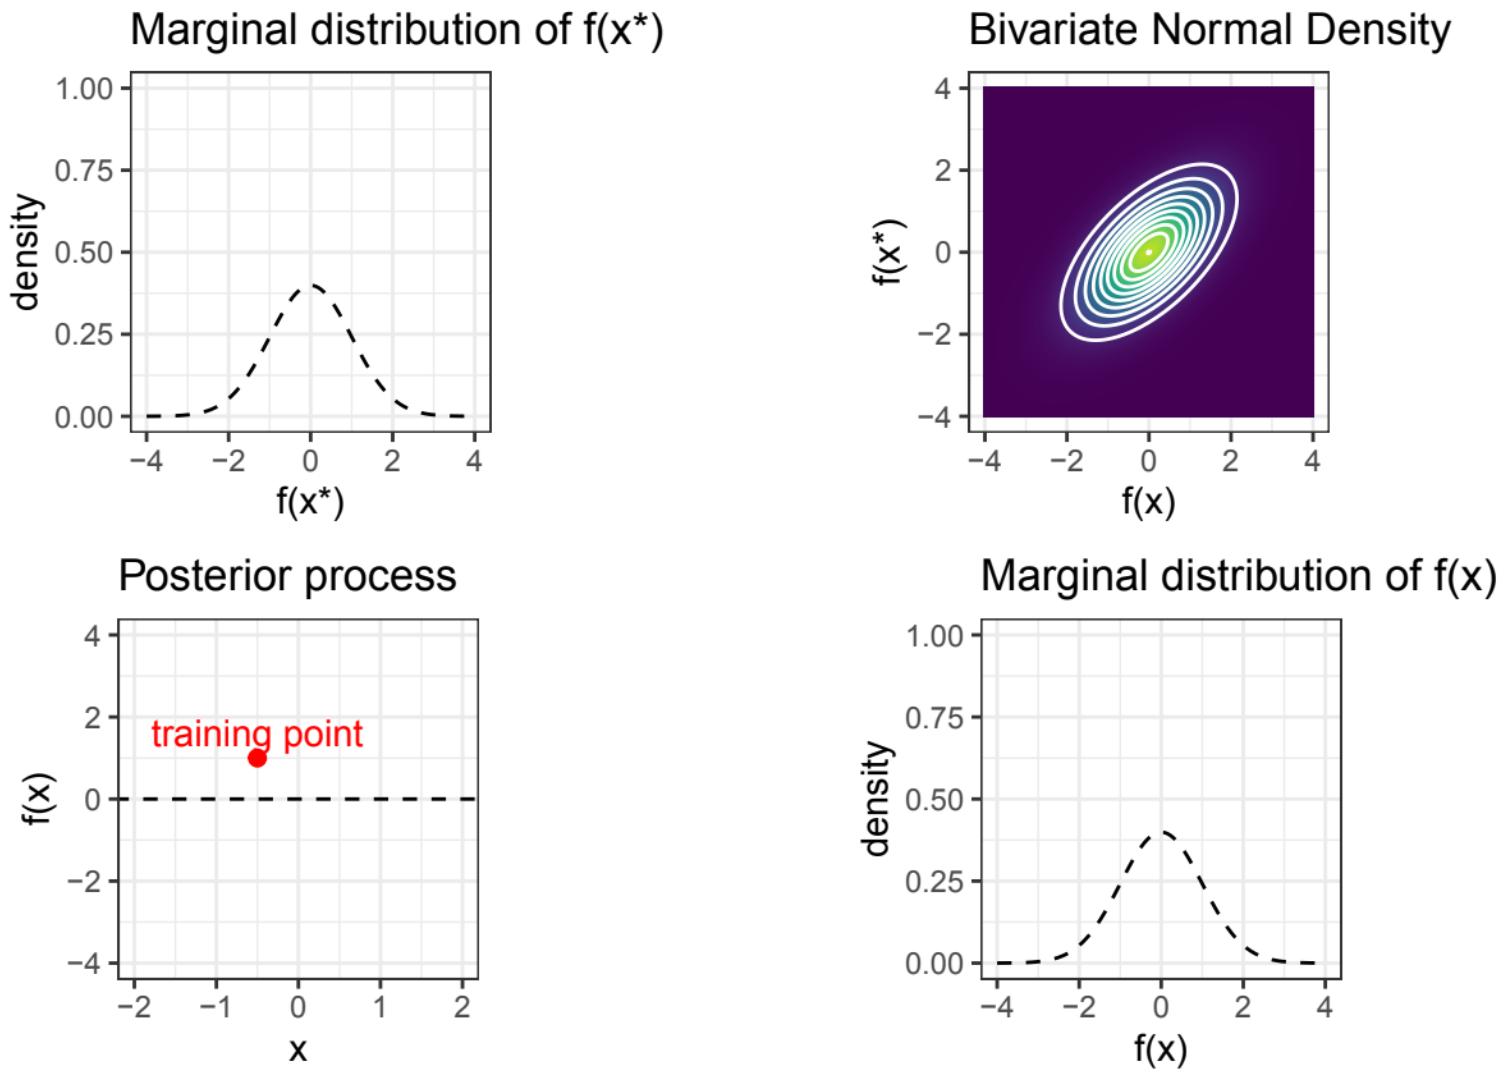
\includegraphics[width=0.8\textwidth]{figure_man/GP02.png}
\end{figure}

\end{frame}
\begin{frame}{GP prediction: Two points}

\begin{footnotesize}
  We condition the Gaussian on $\fx = 1$.
\end{footnotesize}\vspace*{0.2cm}

\begin{figure}
  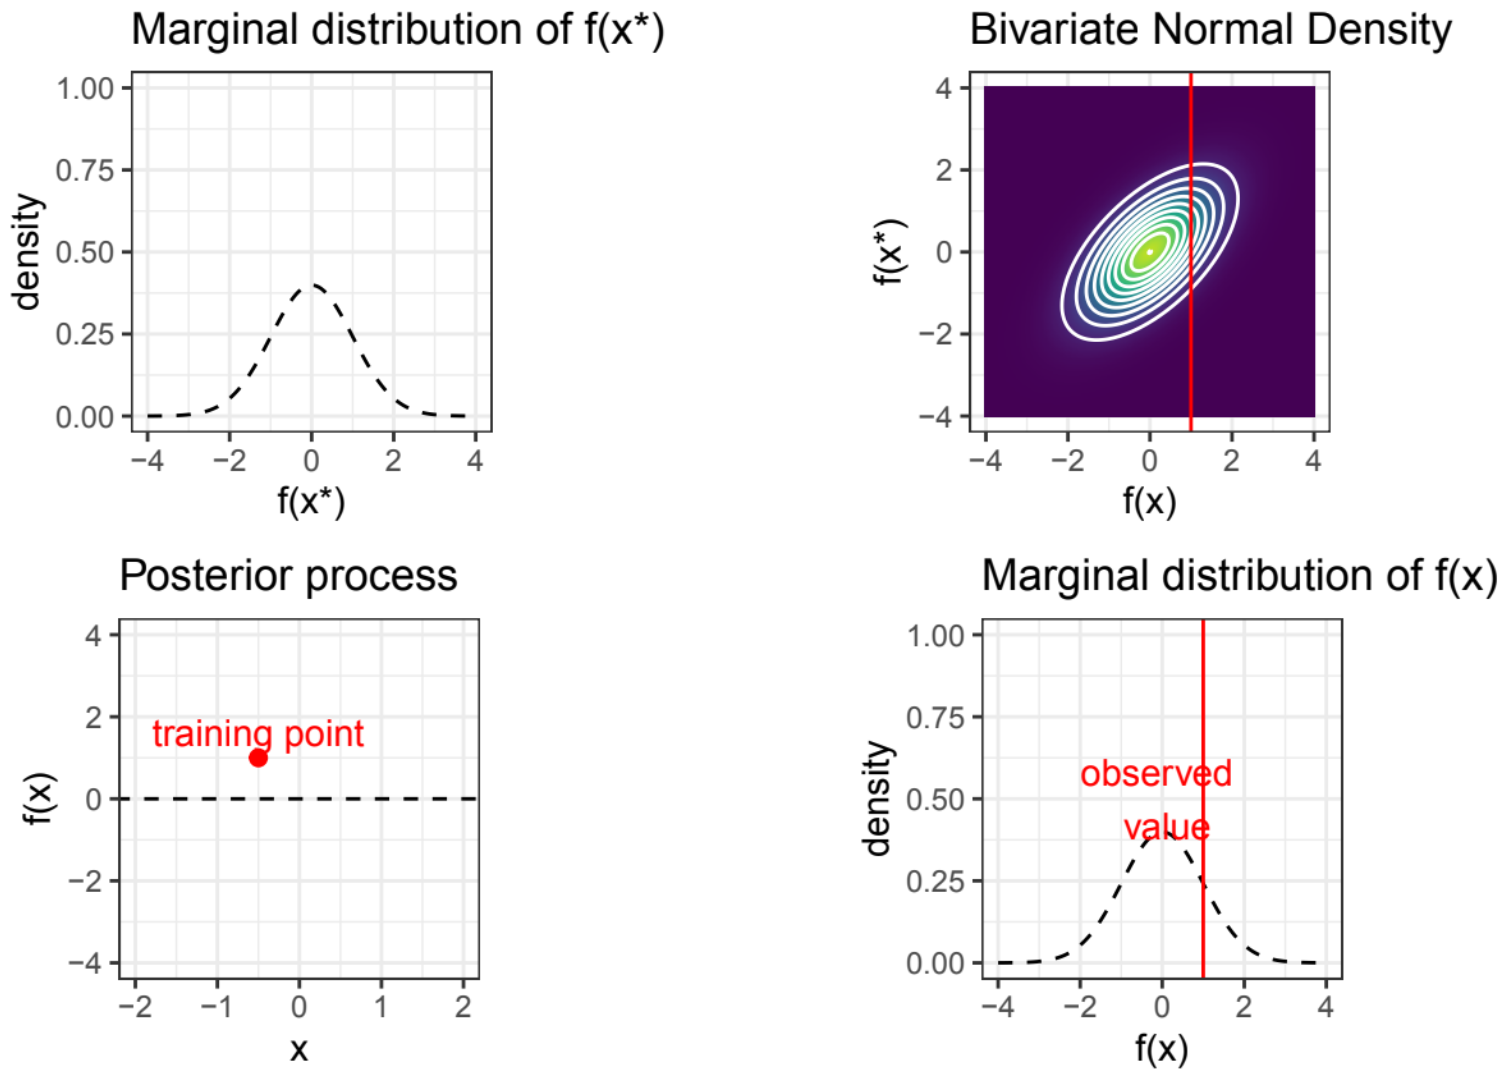
\includegraphics[width=0.8\textwidth]{figure_man/GP03.png}
\end{figure}

\end{frame}


\begin{frame}{GP prediction: Two points}

\begin{footnotesize}
  We compute the posterior distribution of $f(\xv_*)$ given that $\fx = 1$. 
\end{footnotesize}\vspace*{0.2cm}


\begin{figure}
  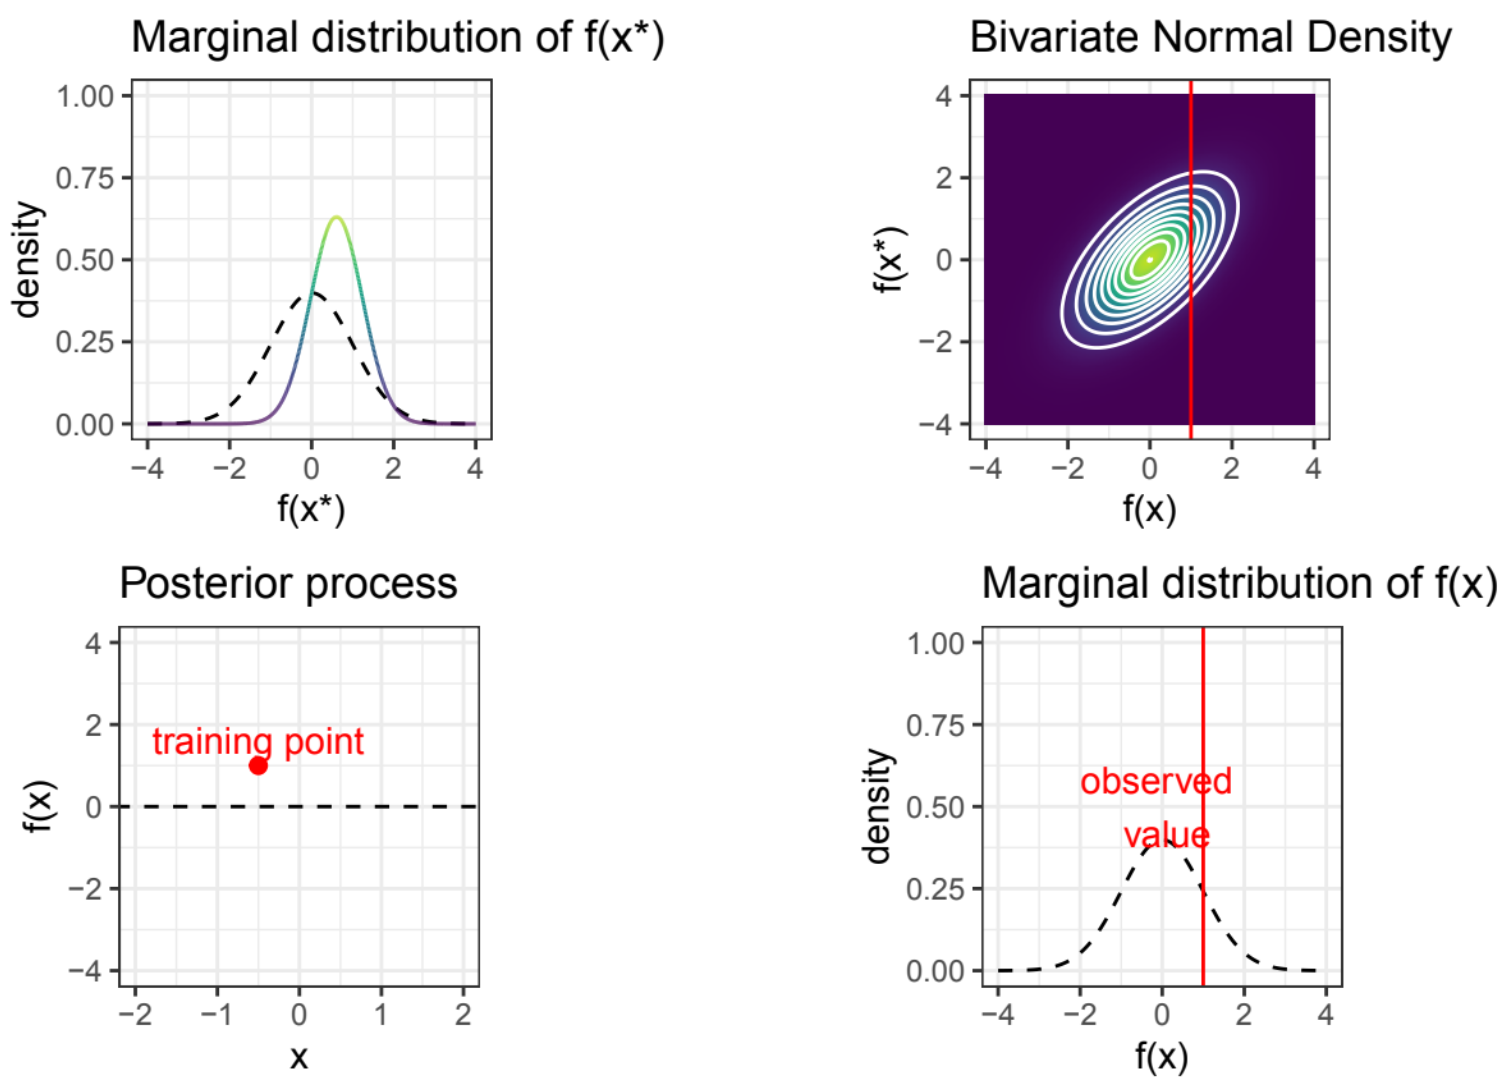
\includegraphics[width=0.8\textwidth]{figure_man/GP04.png}
\end{figure}


\end{frame}
\begin{frame}{GP prediction: Two points}

\begin{footnotesize}
  A possible predictor for $f$ at $\xv_*$ is the MAP of the posterior distribution.
\end{footnotesize}\vspace*{0.2cm}

\begin{figure}
  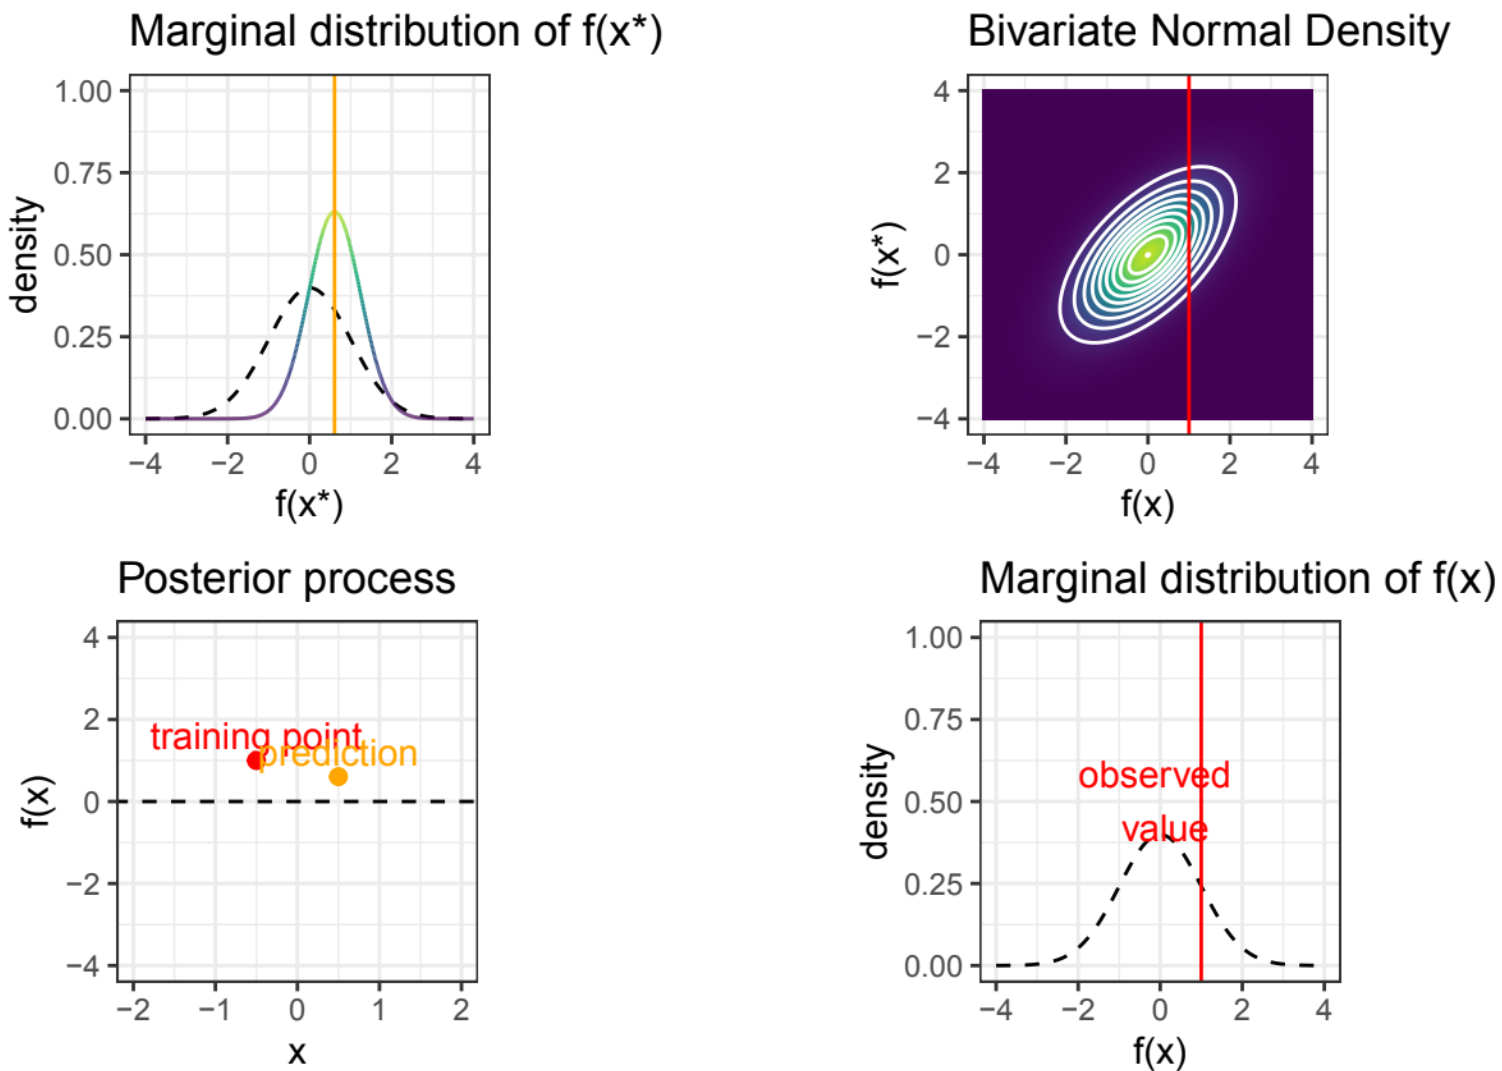
\includegraphics[width=0.8\textwidth]{figure_man/GP05.png}
\end{figure}


\end{frame} 

\begin{frame}{GP prediction: Two points}

\begin{footnotesize}
  We can do this for different values $\xv_*$, and show the respective mean (grey line) and standard deviations (grey area is mean $\pm 2 \cdot $ posterior standard deviation). 
\end{footnotesize}\vspace*{0.2cm}


\begin{figure}
  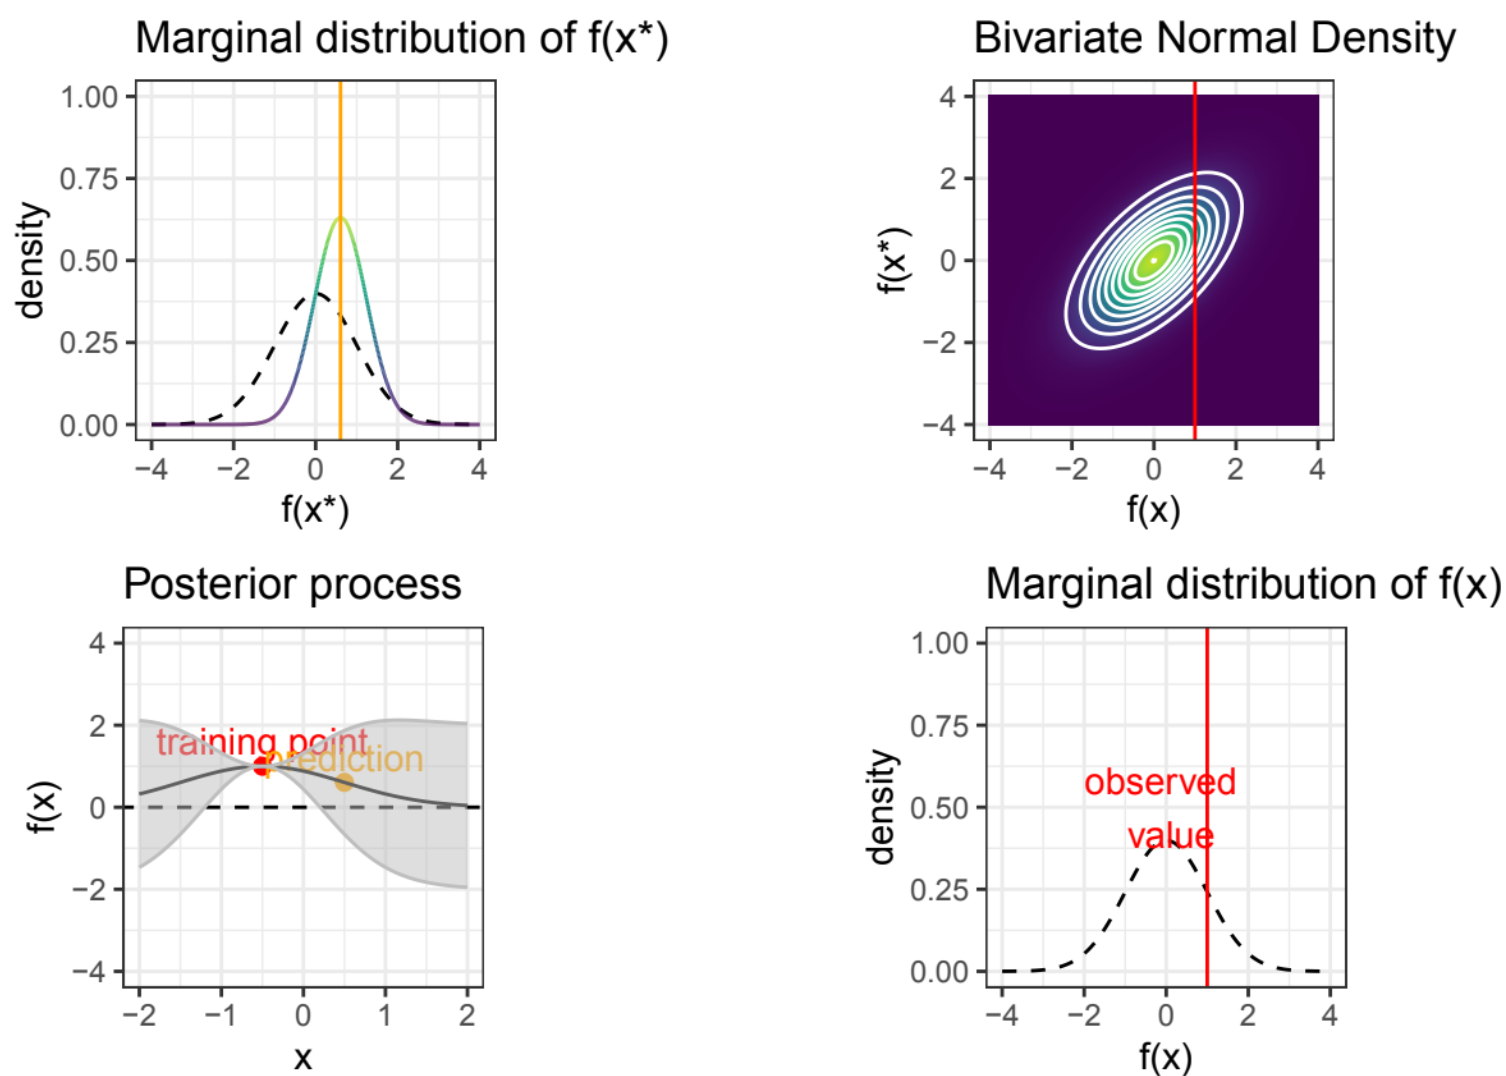
\includegraphics[width=0.8\textwidth]{figure_man/GP06.png}
\end{figure}

\end{frame}

\begin{vbframe}{Posterior Process}

\begin{itemize}
  \item We can generalize the formula for the posterior process for multiple unobserved test points: 

$$
  \bm{f}_* = \left[f\left(\xi[1]_*\right), ..., f\left(\xi[m]_*\right)\right]. 
$$
  \item Under a zero-mean Gaussian process, we have
  $$
    \begin{bmatrix}
    \bm{f} \\
    \bm{f}_*
    \end{bmatrix} \sim  
    \mathcal{N}\biggl(\bm{0}, \begin{bmatrix} \Kmat & \Kmat_* \\ \Kmat_*^T & \Kmat_{**} \end{bmatrix}\biggr),
  $$
    with $\Kmat_* = \left(k\left(\xi, \xv_*^{(j)}\right)\right)_{i,j}$, $\Kmat_{**} = \left(k\left(\xi[i]_*, \xi[j]_*\right)\right)_{i,j}$.
  
  \framebreak 
  
  \item Similar to the single test point situation, to get the posterior distribution, we exploit the general rule of conditioning for Gaussians:
  \begin{eqnarray*}
    \bm{f}_* ~|~ \Xmat_*, \Xmat, \bm{f} \sim \mathcal{N}(\Kmat_{*}^{T}\Kmat^{-1}\bm{f}, \Kmat_{**} - \Kmat_*^T \Kmat ^{-1}\Kmat_*).
  \end{eqnarray*}  
  \item This formula enables us to talk about correlations among different test points and sample functions from the posterior process. 
\end{itemize}

\end{vbframe}


\section{Properties of a Gaussian Process}

\begin{vbframe}{GP as interpolator}

The \enquote{prediction} for a training point $\xi$ is the exact function value $\fxi$

\vspace*{-0.8cm}

\begin{eqnarray*}
\bm{f} ~|~ \Xmat, \bm{f} \sim \mathcal{N}(\Kmat\Kmat^{-1}\bm{f}, \Kmat - \Kmat^T \Kmat^{-1} \Kmat) = \mathcal{N}(\bm{f}, \bm{0}).
\end{eqnarray*}

Thus, a Gaussian process is a function \textbf{interpolator}.

\begin{center}
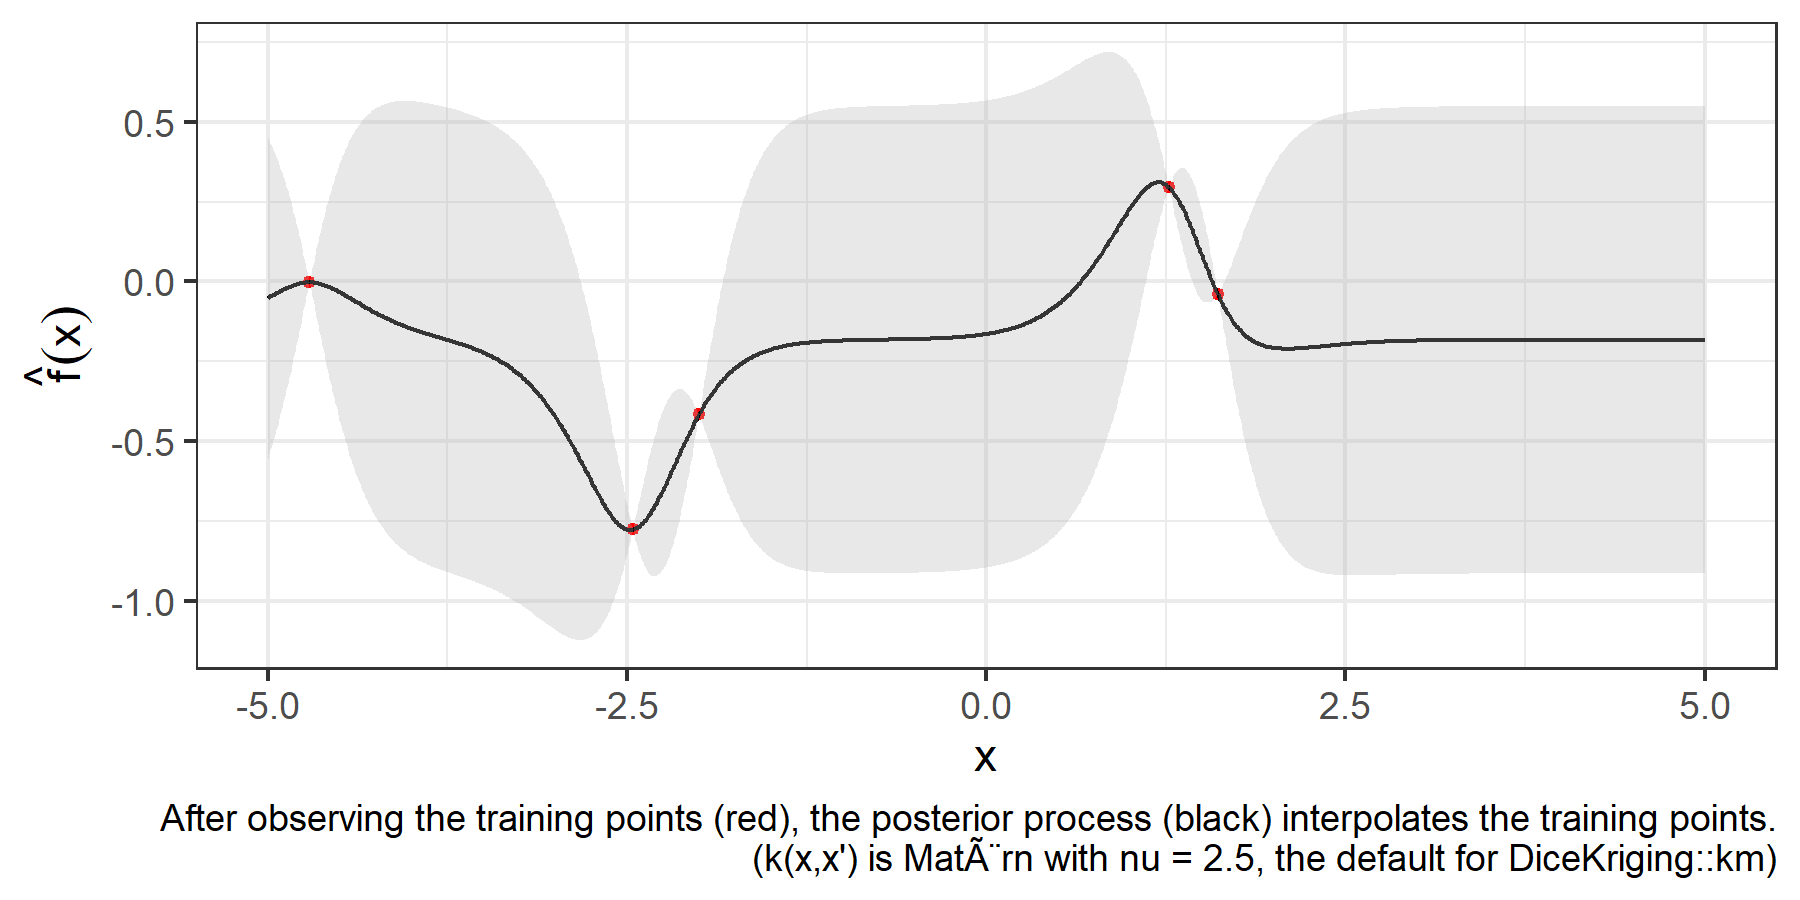
\includegraphics[width=0.8\textwidth]{figure_man/gp-interpolator.png}
\end{center}
% \begin{footnotesize}
% A the posterior process (black) after observing the training points (red) interpolates the training points. 
% \end{footnotesize}

\end{vbframe}


\begin{vbframe}{GP as a spatial model}

\vspace*{-0.3cm}

\begin{itemize}
  \begin{footnotesize}
  \item The correlation among two outputs depends on distance of  the corresponding input points  $\xv$ and $\xv^\prime$ (e.g. Gaussian covariance kernel $k(\xv, \xv^\prime) = \exp \left(\frac{- \|\xv - \xv^\prime\|^2}{2 l^2}\right)$ )
  \item Hence, close data points with high spatial similarity $k(\xv, \xv^\prime)$ enter into more strongly correlated predictions: $\bm{k}_*^\top \bm{K}^{-1} \bm{f}$ ($\bm{k}_* := \left(k(\xv, \xv^{(1)}), ..., k(\xv, \xv^{(n)})\right)$).
  \end{footnotesize}  


\begin{center}
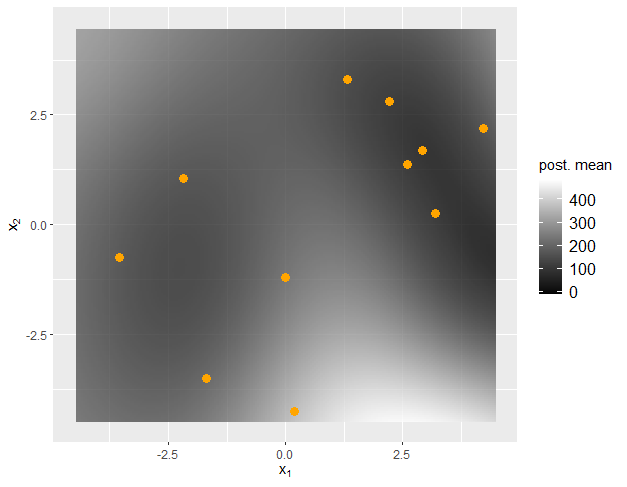
\includegraphics[width=0.4\textwidth]{figure_man/post-mean.png}
\end{center}


\begin{footnotesize}
Example: Posterior mean of a GP that was fitted with the Gaussian covariance kernel with $l = 1$. 
\end{footnotesize}


\framebreak 

\item Posterior uncertainty increases if the new data points are far from the design points.
\item The uncertainty is minimal at the design points, since the posterior variance is zero at these points.
\end{itemize}


\begin{center}
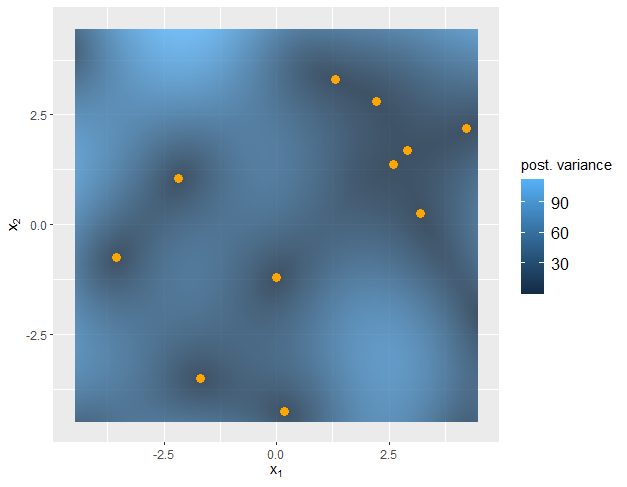
\includegraphics[width=0.4\textwidth]{figure_man/post-variance.png}
\end{center}

\begin{footnotesize}
Example (continued): Posterior variance. 
\end{footnotesize}


\end{vbframe}


\section{Noisy Gaussian Process}

\begin{vbframe}{Noisy Gaussian Process}

\begin{itemize}
  \item So far, we implicitly assumed that we had access to the true function value $\fx$.
  \item For the squared exponential kernel, for example, we have
  $$
    \cov\left(f(\xi), f(\xi)\right) = 1.
  $$
  \item As a result, the posterior Gaussian process is an interpolator: 
  \begin{center}
    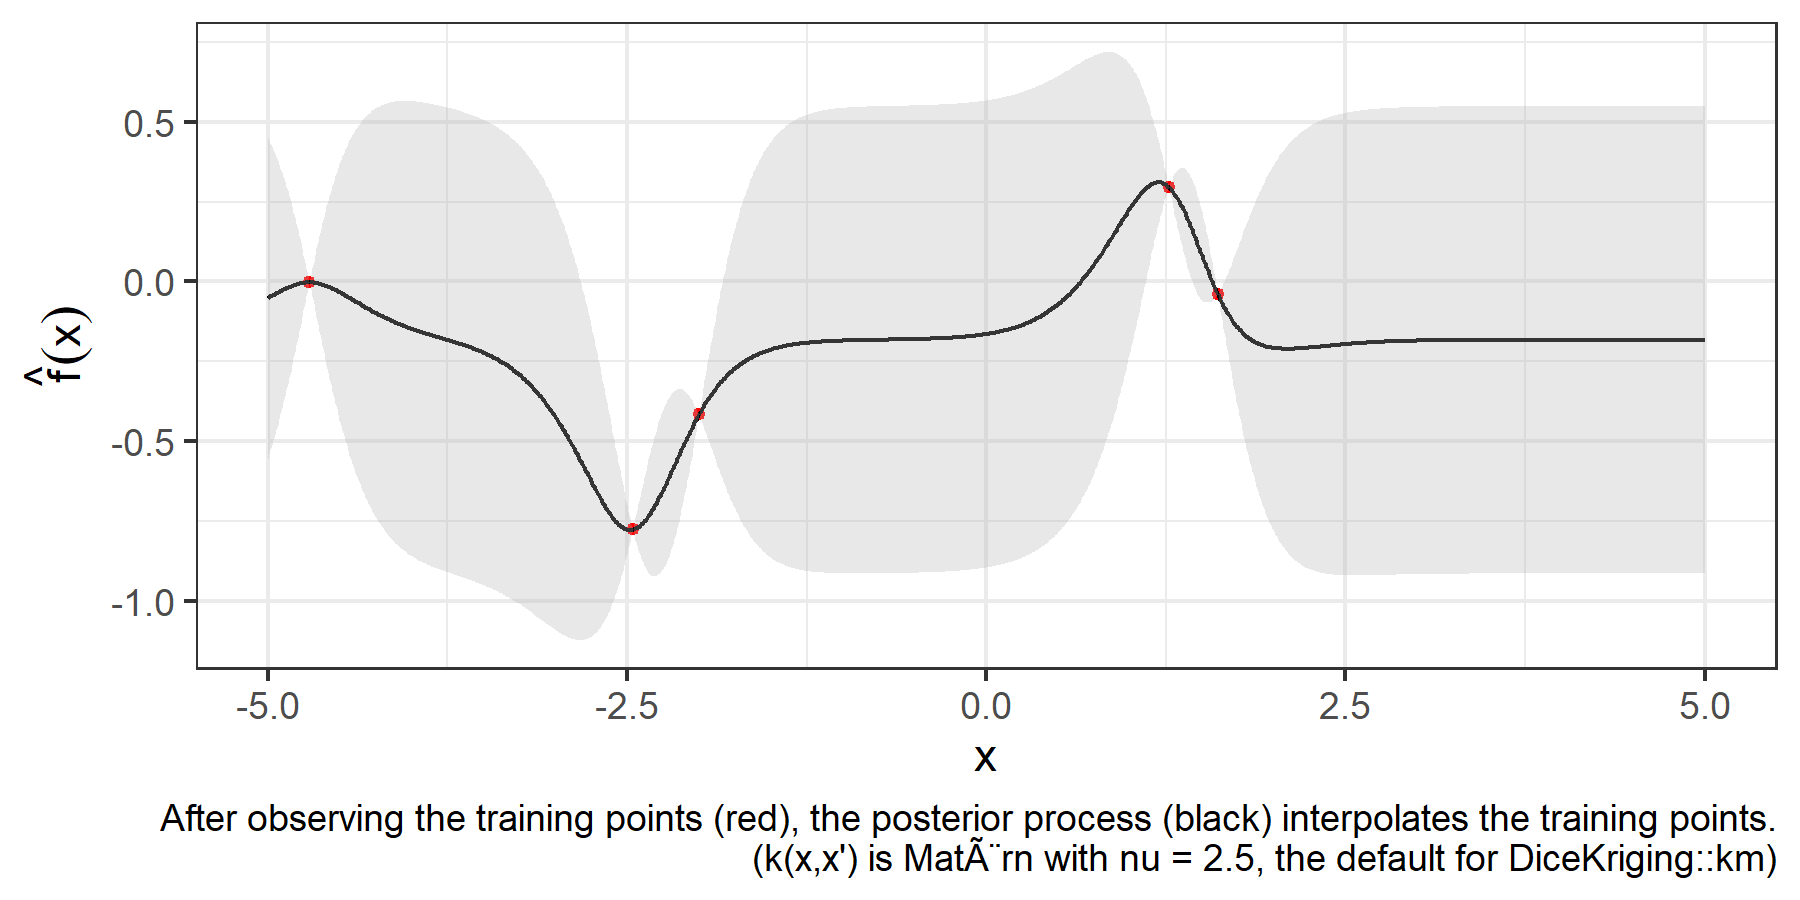
\includegraphics[width=0.8\textwidth]{figure_man/gp-interpolator.png}
  \end{center}

\framebreak 

  \item In reality, however, this is often not the case. 
  \item We often only have access to a noisy version of the true function value
  $$
    y = \fx + \eps, \eps \sim\mathcal{N}\left(0, \sigma^2\right).
  $$
  \item Let us still assume that $\fx$ is a Gaussian process.
  \item Then,
  \begin{footnotesize} 
  \begin{eqnarray*}
    &&\cov(y^{(i)}, y^{(j)}) = \cov\left(f\left(\xi\right) + \epsilon^{(i)}, f\left(\xi[j]\right) + \epsilon^{(j)}\right) \\
    &=& \cov\left(f\left(\xi\right), f\left(\xi[j]\right)\right) + 2 \cdot \cov\left(f\left(\xi\right), \epsilon^{(j)}\right) + \cov\left(\epsilon^{(i)}, \epsilon^{(j)}\right) 
    \\ &=& k\left(\xi, \xi[j]\right) + \sigma^2 \delta_{ij}. 
  \end{eqnarray*}
  \end{footnotesize}
  \item $\sigma^2$ is called \textbf{nugget}. 
\end{itemize}

\framebreak 

\begin{itemize}
  \item Let us now derive the predictive distribution for the case of noisy observations. 
  \item The prior distribution of $y$, assuming that $f$ is modeled by a Gaussian process is then
  $$
    \bm{y} = \begin{pmatrix} \yi[1] \\ \yi[2] \\ \vdots \\ \yi[n] \end{pmatrix} \sim \mathcal{N}\left(\bm{m}, \bm{K} + \sigma^2 \bm{I}_n \right),
  $$
  with 
  \begin{eqnarray*}
    \textbf{m} &:=& \left(m\left(\xi\right)\right)_{i}, \quad
    \textbf{K} := \left(k\left(\xi, \xv^{(j)}\right)\right)_{i,j}. 
  \end{eqnarray*}

  \framebreak 
  
  \item We distinguish again between 
  \begin{itemize}
    \item observed training points $\Xmat, \yv$, and 
    \item unobserved test inputs $\Xmat_*$ with unobserved values $\bm{f}_*$
  \end{itemize} 
  and get
  $$
  \begin{bmatrix}
  \bm{y} \\
  \bm{f}_*
  \end{bmatrix} \sim  
    \mathcal{N}\biggl(\bm{0}, \begin{bmatrix} \Kmat + \sigma^2 \bm{I}_n & \Kmat_* \\ \Kmat_*^T & \Kmat_{**} \end{bmatrix}\biggr).
  $$

\framebreak

  \item Similarly to the noise-free case, we condition according to the rule of conditioning for Gaussians to get the posterior distribution for the test outputs $\bm{f}_*$ at $\Xmat_*$: 

  \begin{eqnarray*}
    \bm{f}_* ~|~ \Xmat_*, \Xmat, \bm{y} \sim \mathcal{N}(\bm{m}_{\text{post}}, \bm{K}_\text{post}).
\end{eqnarray*}
  with 
  \begin{eqnarray*}
    \bm{m}_{\text{post}} &=& \Kmat_{*}^{T} \left(\Kmat+ \sigma^2 \cdot \id\right)^{-1}\bm{y} \\
    \bm{K}_\text{post} &=& \Kmat_{**} - \Kmat_*^T \left(\Kmat ^{-1} + \sigma^2 \cdot \id\right)\Kmat_*,
  \end{eqnarray*}
\item This converts back to the noise-free formula if $\sigma^2 = 0$.

\framebreak 

\item The noisy Gaussian process is not an interpolator any more.
\item A larger nugget term leads to a wider ``band'' around the observed training points.
\item The nugget term is estimated during training.


\begin{center}
    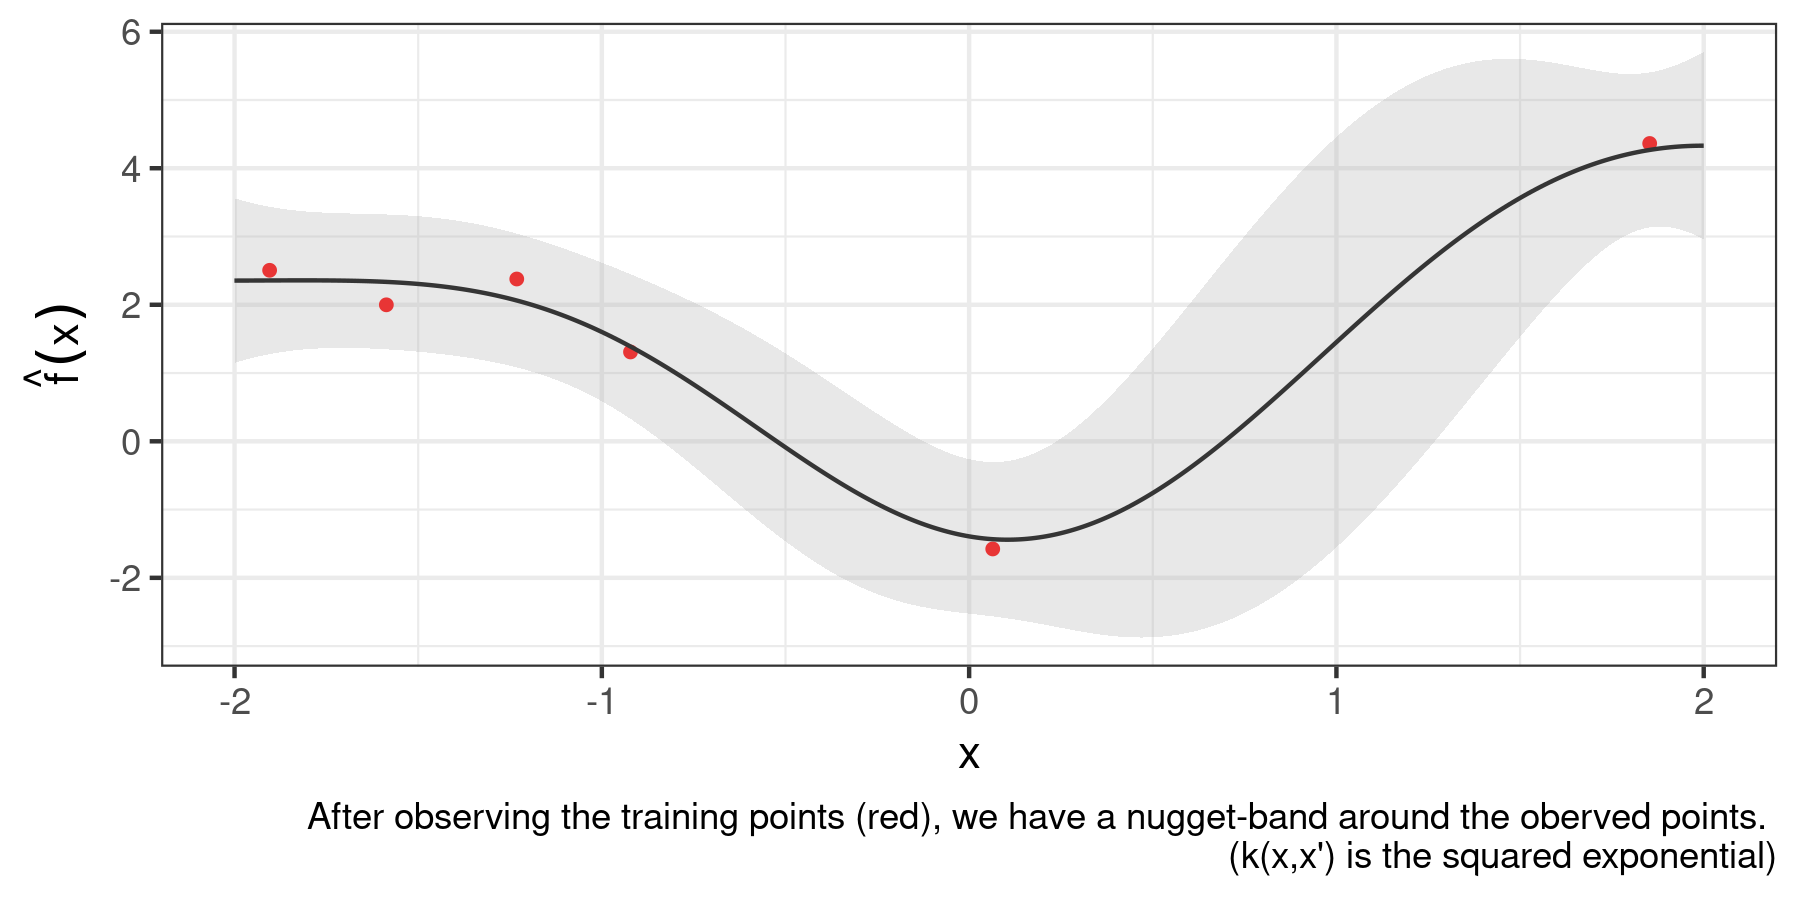
\includegraphics[width=0.8\textwidth]{figure_man/gp-regression.png}
\end{center}
\end{itemize}

\end{vbframe}



\section{Decision Theory for Gaussian Processes}

\begin{vbframe}{Risk Minimization for Gaussian Processes}

In machine learning, we learned about risk minimization. We usually choose a loss function and minimize the empirical risk  

$$
  \riske(f) := \sumin \Lxyi
$$
as an approximation to the theoretical risk

$$ 
  \riskf := \E_{xy} [\Lxy] = \int \Lxy \text{d}\Pxy. 
$$

\begin{itemize}
  \item How does the theory of Gaussian processes fit into this theory? 
  \item What if we want to make a prediction which is optimal w.r.t. a certain loss function? 
\end{itemize}

\framebreak 

\begin{itemize}
  \item The theory of Gaussian process gives us a posterior distribution 
  $$
    p(y ~|~\D)
  $$
  \item If we now want to make a prediction at a test point $\bm{x}_*$, we approximate the theoretical risk in a different way, by using the posterior distribution: 
  $$
    \mathcal{R}(y_* ~|~ \bm{x}_*) \approx \int L(\tilde y_*, y_*) p(\tilde y_*~|~\bm{x}_*, \D)d\tilde y_*. 
  $$
  \item The optimal prediciton w.r.t the loss function is then: 
  $$
    \hat y_* | \bm{x}_* = \argmin_{y_*} \mathcal{R}(y_*~|~ \bm{x}_*).
  $$
\end{itemize}


% In practical applications, we are often forced to make predictions. We need a point-like prediction that is \enquote{optimal} in some sense. 

% \lz

% We define \enquote{optimality} with respect to some loss function

% $$
% L(y_\text{true}, y_\text{guess}). 
% $$

% \vfill

% \begin{footnotesize}
% Notice that we computed the predictive distribution without reference to the loss function. In non-Bayesian paradigms, the model is typically trained by minimizing the empirical risk (or loss). In contrast, in the Bayesian setting there is a clear separation between the likelihood function (used for training in addition to the prior) and the loss function.
% \end{footnotesize}

% \framebreak 

% As we do not know the true value $y_\text{true}$ for our test input $\bm{x}_*$, we minimize w.r.t. to the expected loss called \textbf{risk} w.r.t. our model's opinion as to what the truth might be

% $$
% \mathcal{R}(y_\text{guess} | \bm{x}_*) = \int L(y_*, y_\text{guess}) p(y_*|\bm{x}_*, \D)dy_*. 
% $$

% Our best guess w.r.t. $L$ is then

% $$
% $$

% For quadratic loss $L(y, y^\prime) = (y - y^\prime)^2$ this corresponds to the posterior mean. 

\end{vbframe}


\endlecture
\end{document}
